% !TEX root = ../Documentation.tex

\section{Design}
\label{sec:design}

\subsection{System overview (D)}
  The parser module overview is given in \autoref{fig:ParserModules}.
  Each of the modules are described in the following subsection.
  %
  \begin{figure}[ht]%
    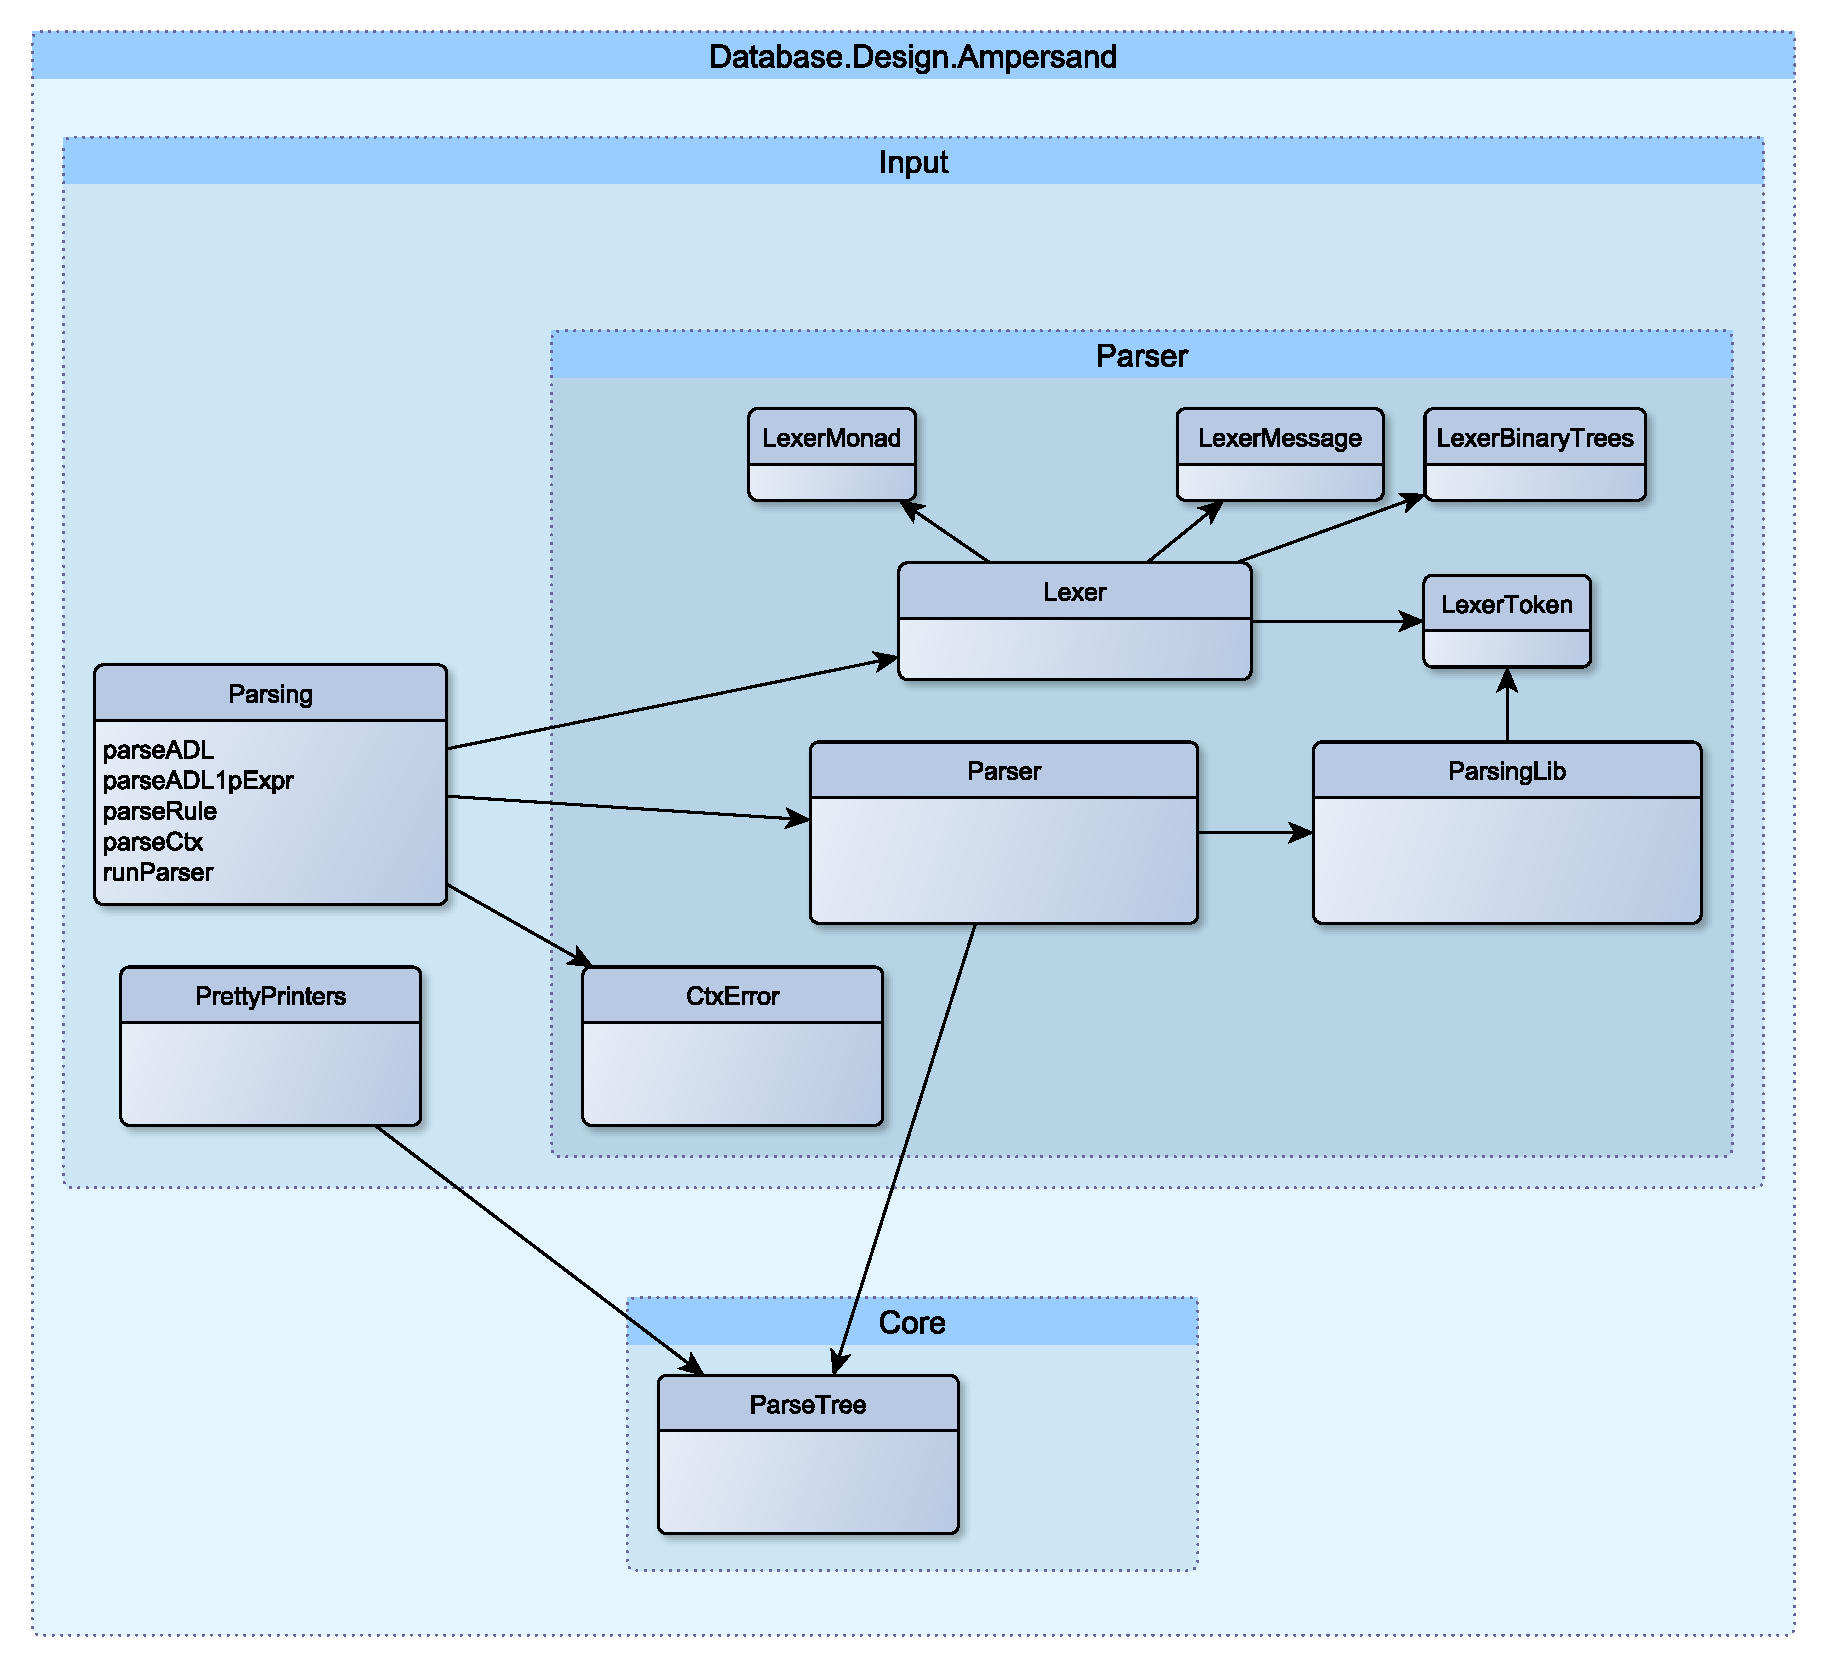
\includegraphics[width=\columnwidth]{Figures/ParserModules}
    \caption{The parser modules and their relationships}
    \label{fig:ParserModules}
  \end{figure}%
  TODO: Add the exported functions to each module.

  \subsubsection{Modules}
  \label{subsec:parser-modules}
  In this section a short description of each module is given:
  %
  \begin{description}
    \item[Parsing] module that implements the interface of the parser with the rest of the system.
      It is responsible for reading the input files, calling the lexer and the parser and returning a parse tree as result (or a parse error).

    \item[Parser] module responsible for executing the parsing itself.
      It accepts the tokens that are allowed in each grammar production and generates the corresponding parse tree.
      The parser is described in \autoref{subsec:design-parser}.
      
    \item[ParsingLib] library that contains several useful functions to assist the parser, e.g. token recognition.
      These functions are not depending on the specific grammar rules.
      
    \item[ParseTree] external module containing the parse tree data structures.
      Only details of this module have been changed during this project (e.g. field ordering).
    
    \item[PrettyPrinters] contains the \texttt{Pretty} class and the functions responsible for printing the parse tree to ADL scripts in a `pretty' way.
    
    \item[CtxError] contains the data structures responsible for the parse errors and their location.
      This module has not been refactored as a part of this project.
    
    \item[Lexer] module responsible for recognizing the input characters and converting them to tokens.
      The lexer, together with its sub-modules, is described in \autoref{subsec:lexer}.
  \end{description}

\subsection{Lexer (M)}
\label{subsec:lexer}

\subsubsection{The rationale behind the new lexer}
In the design of the new Ampersand parser, the question arose whether to keep the current scanner, the former name of the lexer module within Ampersand, or to implement a new one.
After the analysis of the error improvement areas, as described in \autoref{sec:analysis}, the main improvements were identified within the actual parser.
The error feedback quality produced by the scanner module was higher and therefore, there was no stringent need to re-implement the scanner.
On the other hand, given the aspect that Parsec was defined as the new parser library, keeping the current scanner would have resulted in the utilization of 2 different libraries providing more of less the same functionality.
Besides the error message quality, other improvement topics were identified in \autoref{subsec:analysis-lexer}.
To avoid a decrease in maintainability, the decision is made to implement the parser and scanner based on the same library.
During the implementation of the lexer module, replacing the old scanner, additional attention was given to further improve the quality of the error messages.
The scanner module is renamed to the lexer module to stress the aspect that the principle of lexemes is used in the new scanner.
Lexemes can be seen as the part of a token containing the actual language content besides the actual position information.

The lexer is build based on the existing Helium lexer modules. 
One of the main goals of this project create a compiler and a dialect of Haskell in which clear error messages were produced. TODO: reference
The lexer module in Helium contains interesting principles such as position monitoring, warnings and easy maintainable error messages.


\subsubsection{Lexer structure}

The lexer is the main module, in which the actual lexing is done, and to do so, it it using the following sub-modules:

 \begin{description}
 
    \item[LexerMonad] contains a monad definition that supports lexing with context.
      It tracks for example the location in the input and the warnings that may be generated.
	  This module is re-used without any modification out of the  Helium parser.
      The following functions or types are used in the Ampersand lexer:
	  \begin{itemize}
		\item [LexerMonad] is the main monadic type used in the lexer returning an error or a list of tokens together with a list of warnings
		\item [addPos] is used to trace the position of the token
		\item [lexerError] to generate lexer error
		\item [lexerWarning] to generate lexer warnings
		\item [runLexerMonad] main function to handle the LexerMonad results 
	  \end{itemize}
	  
    \item[LexerMessage] contains functions to handle errors and warnings from the lexer.
	  Based on the warning/error type and the needed language, LexerMessage will fetch the correct description of an error or a warning out of the LexerTexts module
	  The show functions for the error and warning are maintained in this module.
	  
    \item[LexerTexts] will fetch the correct description of an error or a warning out of the LexerTexts module.
	  This centralisation provides an easy entry point for the maintenance of the actual messages as the actual messages are no longer dispersed over the module functions.
	  
    \item[LexerBinaryTrees] module responsible for searching binary trees in an efficient way, to support the token recognition.
            This is the existing UU\_BinaryTrees module which is renamed to match the used naming structure of the new lexer modules.

    \item[LexerToken] contains the data structure, and corresponding show function, that represents the input tokens for the lexer.
	
  \end{description}


\subsubsection{New token structure}
Based on the improvement topics mentioned in \autoref{subsec:analysis-lexer}, a new token structure is defined.

Each token contains the lexeme: a part of the input string together with an identifier, defining the token content, and the position of the token in the input file.
The token structure is defined as follows:


\begin{verbatim}
  data Token = Tok {	  tokLex :: Lexeme
                		    , tokPos :: FilePos   }
\end{verbatim}

The lexeme is the combination of the token type and the actual token content, sliced from the input string.
FilePos is used to keep track of the original position of the lexeme in the input string.

During the lexer processing, the input file is processed sequentially.
All kind of differentiating formats are checked in a specific order, and each time a match is found, the lexeme is extracted from the input file and the token is created.
In the token creation, function \texttt{ReturnToken}, the position and lexeme is grouped into the actual token and the next nested lexer iteration is launched.

\subsection{Parser (R-M)}
\label{subsec:design-parser}
The mainstream design of the new parser has not changed much.
Basically, each EBNF rule receives its own parser function.
Thanks to the combinator operators, each parsing function also looks very similar to its corresponding EBNF.

The applicative interface is consistently used.
By changing details of the implementation, e.g. the order of the fields in the parse tree, we have made many of the `rebuild' functions unnecessary.
For some parsers the amount of changes necessary in order to remove supporting functions was too large or even impossible with the current parse tree.

Note that in parts of the parser, the function syntax has substituted the record syntax for creating data objects.
This was done only when the code readability could be improved by doing so.

\subsubsection{Parsec}
\label{subsec:design-parsing-lib}
As mentioned earlier, and described in research context document \citenac{parsing}, the new Ampersand parser has been rebuilt with another parsing library, namely Parsec.
However, for the Ampersand developers, the source code of the parser will still look very familiar, thanks to the applicative interface.
For developers, the main differences between Parsec and the uulib are:
\begin{itemize}
  \item Parsec does not backtrack by default.
    In order to enable backtracking, the \texttt{try} function must be used.
    This is described in \autoref{subsec:backtracking}.
  \item Parsec does not try to solve parsing errors.
    The parser stops immediately after the first issue.
    See also the error analysis in \autoref{subsec:design-errors}.
  \item Error messages are customizable by using the \texttt{<?>} operator.
    This is also suggested in \autoref{subsec:design-next-steps}.
  \item Some combinators have a different name, e.g. one must use \texttt{option} instead of \texttt{opt}.
    Assuming the documentation found on Hackage is clear and sufficient, interface differences are not documented here.
\end{itemize}

\subsubsection{Backtracking}
\label{subsec:backtracking}
In order to explain the differences on backtracking behavior between the uulib and Parsec, we quote here Doaitse Swierstra, the author of the uulib \citenac{swierstra-parsec}:
\begin{quote}
\textsl{To understand the subtleties it is important to understand the differences between the try construct in Haskell and the non-greedy parsing strategy used in uu-parsinglib. Effectively the latter is a try which just looks ahead one symbol. In that respect it is less powerful than the try construct from Parsec, in which you specify that a specific construct has to be present completely. And then there is the underlying different overall strategy. Parsec uses a back-tracking strategy with explicit tries to commit, whereas uu-parsinglib uses a breadth-first strategy with an occasional single symbol look-ahead.}
\end{quote}
%
We can therefore conclude that the try-statements in Parsec are undesirable.
However, they are necessary when the grammar is ambiguous.
In this section we explain why each of the remaining try statements are necessary, and how these issues can be resolved:
\begin{description}
  \item[Classify]
    This ambiguity in the grammar arises from the \texttt{Classify} and \texttt{GenDef} productions:
    \begin{quote}
        \texttt{Classify ::= `CLASSIFY' ConceptRef `IS' Cterm}\\
        \texttt{GenDef ::= (`CLASSIFY' | `SPEC') ConceptRef `ISA' ConceptRef}
    \end{quote}
    When the parser encounters \texttt{`CLASSIFY'}, it cannot define whether it found a \texttt{Classify} or a \texttt{GenDef} production.
    Therefore, the parser must consume the keyword and a \texttt{ConceptRef} before consuming either \texttt{`IS'} or \texttt{`ISA'} and determining which production is applicable.
    
    In order to solve this issue, one must choose a different keyword or symbol for each of the productions.
    Another option would be to merge the two statements in the same parser.
    We did not merge the productions because that would make the parser less maintainable.
  
  \item[Role]
    This ambiguity in the grammar arises from the \texttt{RoleRelation} and \texttt{RoleRule} productions:
    \begin{quote}
        \texttt{RoleRelation ::= `ROLE' RoleList `EDITS' NamedRelList}\\
        \texttt{RoleRule ::= `ROLE' RoleList `MAINTAINS' ADLidList}
    \end{quote}
    When the parser encounters \texttt{`ROLE'}, it cannot define whether it is a \texttt{RoleRelation} or a \texttt{RoleRule} production.
    Therefore, the parser must consume the keyword and a \texttt{RoleList} (which may be long) before consuming either \texttt{`MAINTAINS'} or \texttt{`EDITS'} and determining which production is applicable.
    
    In order to solve this issue, one must choose a different keyword for each of the productions, merge the two options to have the same representation in the parse tree, or refactor the parser so that the two options are parsed together.
    We did not merge the productions because that would make the parser less maintainable.
  
  \item[View]
    This ambiguity in the grammar arises from the \texttt{FancyViewDef} and \texttt{ViewDefLegacy} productions:
    \begin{quote}
        \texttt{FancyViewDef ::= `VIEW' Label ConceptOneRefPos `DEFAULT'? `\{' ViewObjList `\}' HtmlView? `ENDVIEW'}\\
        \texttt{ViewDefLegacy ::= (`VIEW' | `KEY') LabelProps ConceptOneRefPos `(' ViewSegmentList `)' }
    \end{quote}
    When the parser encounters \texttt{`VIEW'}, it cannot define whether it found a \texttt{FancyViewDef} or a \texttt{ViewDefLegacy} production.
    In this case, defining which construction is applicable is even more complicated.
    This decision must, in the worst case, be delayed until the parser encounters a \texttt{`\{'} or \texttt{'('}.
    That's because the productions \texttt{Label} and \texttt{LabelProps} are not disjoint, and \texttt{`DEFAULT'} is optional.
    
    In order to solve this issue, we advise to merge or drop the legacy statement.
    
  \item[Multiplicity]
    This ambiguity in the grammar arises from the \texttt{Mult} production:
    \begin{quote}
        \texttt{Mult ::= (`0' | `1') `..' (`1' | `*') | `*' | `1'}
    \end{quote}
    When the parser encounters \texttt{`1'}, it cannot define whether it found the first or the last production.
    The parser must therefore read the next token before choosing the right option.
    
    In order to solve this issue, we advise to refactor the grammar (and the parser) to have the following production:
    \begin{quote}
        \texttt{Mult ::= `0' `..' (`1' | `*') | `1'(`..' (`1' | `*'))? | `*'}
    \end{quote}
    %
    We did not refactor the code in this manner because the \texttt{pMult} parser does more than only parsing: it also changes the representation of the found constructions before creating the parse tree.
  
  \item[Labels and Terms]
    In the productions \texttt{Att} and \texttt{RuleDef}, we see very similar ambiguities:
    \begin{quote}
        \texttt{Att ::= LabelProps? Term}\\
        \texttt{RuleDef ::= `RULE' Label? Rule Meaning* Message* Violation?}
    \end{quote}
    Wherein:
    \begin{quote}
        \texttt{Label ::= ADLid ':'}\\
        \texttt{LabelProps ::= ADLid (`{' ADLidListList `}')? `:'}\\
        \texttt{Rule ::= Term ('=' Term | '|-' Term)?}
    \end{quote}
    And one of the possible productions of \texttt{Term} is:
    \begin{quote}
        \texttt{Term ::= Trm2 ::= Trm3 ::= Trm4 ::= Trm5 ::= Trm6 ::= RelationRef ::= NamedRel ::= Varid Sign?}
    \end{quote}
    While:
    \begin{quote}
        \texttt{ADLid ::= Varid | Conid | String}
    \end{quote}
    
    What happens here is that when the parser encounters a \texttt{Varid}, it cannot define whether it is part of the (optional) \texttt{Label} production or if no \texttt{Label} was given and the \texttt{Varid} is part of a \texttt{Term}/\texttt{NamedRel} production.
    
    Due to the quite complex grammar for the \texttt{Term} production, this issue may severely impact the parser's performance.
    This is probably the most harmful of the ambiguities mentioned.
    However, it can only be solved by adding a symbol before the \texttt{Term} production (e.g. making the `:' non-optional).
\end{description}
%
Please note that in order to have proper backtracking with correct error messages, Parsec may require two try-statements \citenac{try-harmful}.

\subsection{Parse tree (R-M)}
\label{subsec:design-parse-tree}
Improvements in the Ampersand parse tree are out of the scope of this project, because of the potential consequences to the rest of the Ampersand system.
However, during the development of the new parser a few constructions have been changed in order to make the parser more readable and maintainable.
The changes have been mostly in the order of the constructor parameters, and this was done consequently though all Ampersand modules.
The updated parse tree is depicted in the appendices (\autoref{fig:parse-tree}).

\subsection{Errors (M)}
\label{subsec:design-errors}
The proof of the pudding is in the eating, and therefore, our error message qualification definition from \autoref{subsec:analysis-errors} is applied on the new parser.
All erroneous syntax statements recorded during the analysis phase are fed to the new parser to draw up the error message quality overview of the new parser.

The results are placed in the overview below next to the results of the old parser as a reference point.
The actual error list, containing the syntax statements with the corresponding error messages, is available as an appendix to this document.

% Please add the following required packages to your document preamble:
% \usepackage[table,xcdraw]{xcolor}
% If you use beamer only pass "xcolor=table" option, i.e. \documentclass[xcolor=table]{beamer}
\begin{table}[h]
  \centering
	\begin{tabular}{llrlr}
    Error quality  & \multicolumn{2}{c}{Old parser} & \multicolumn{2}{c}{New parser} \\
		Good           & 19          & 22,35\%          & 70          & 82,35\%          \\
		Average        & 18          & 21,18\%          & 14          & 16,47\%          \\
		Bad            & 48          & 56,47\%          & 1           &  1,18\%          \\
		\rowcolor[HTML]{BBBBBB}
		\textbf{Total} & \textbf{85} & \textbf{100,00\%} & \textbf{85} & \textbf{100,00\%}
	\end{tabular}
  \caption{Error message comparison results}
  \label{tab:error-messages-results}
\end{table}

The table clearly visualizes that there indeed was an issue with the error messages generated by the old Ampersand parser.
By implementing the new parser, an improvement of 360\% is made towards the creation of good error messages in which 82\% of the generated error messages are good, compared to 22\% in the old Parser.

One bad error message remains in the system.
After analysis, the resolution of this remaining bad error would require too much effort, hence increased complexity, compared to the actual value gain.
The error in question is thrown when the \texttt{Meta} statement is used with only one string value. 
Given the simple structure of the notation, we assume that the reference to the line number of the \texttt{Meta} is sufficient although the error message is unclear.
Therefore, this message is kept as is.

\subsection{Next steps (M)}
\label{subsec:design-next-steps}
TODO: give tips on how to further improve the parser. e.g.:
  - cleanup CtxError, add warnings, use <?> for the errors.
  - reorganize parse tree, e.g. using always Origin as first parameter.